\documentclass[a4paper,oneside,12pt]{report}
\usepackage{graphicx}
\usepackage{titlesec}
\usepackage{cite}
\usepackage{setspace}
\usepackage{amsmath}
\usepackage{amssymb}
\usepackage{refstyle}
\usepackage[titletoc]{appendix}

%\usepackage{tocloft}
%\usepackage[Lenny]{fncychap}

\usepackage[a4paper,bindingoffset=0.0mm,%
left=40mm,right=25mm,top=25mm,bottom=40mm,%
footskip=.25in]{geometry}
\usepackage{blindtext}

\renewcommand\contentsname{Table of Contents}

\renewcommand{\baselinestretch}{1} 

\titleformat{\chapter}[display]
{\filleft\normalfont}{\scshape\chaptertitlename\ \thechapter}{-20pt}{\large\bfseries\MakeUppercase}
[\vspace{-3.5ex}
\rule{\textwidth}{0.3pt}]
\titlespacing{\chapter}
{0pt}{10pt}{20pt}
\renewcommand{\chaptername}{Section}

\titleformat{\section}[hang]
{\normalfont\bfseries}{\thesection}{0.5em}{}
\titlespacing{\section}
{0pt}{20pt}{20pt}

\titleformat{\subsection}[hang]
{\normalfont\bfseries}{\thesubsection}{0.5em}{}
\titlespacing{\subsection}
{0pt}{10pt}{10pt}

\titleformat{\subsubsection}[hang]
{\normalfont\bfseries}{\thesubsubsection}{0.5em}{}
\titlespacing{\subsubsection}
{0pt}{10pt}{10pt}


\begin{document}
	
%Title Page
\begin{titlepage}
	\begin{center}
		
\includegraphics[scale=0.5]{uom}
		
		\vspace*{1cm}
		\Large
		\textbf{PdD Research Proposal}
		
		\vspace*{2cm}
		\Huge
		\textbf{Vision Based Navigation for Aerial and Ground Vehicles }
		
		\vspace{1cm}
		\large
		\textbf{M.H.G.D. Tissera}
		
		\vspace{1cm}
		\large
		\textbf{188013F}
		
		\vspace{1.5cm}
		\normalsize
		Supervisors:\\
		Dr. Ranga Rodrigo\\
		Dr. Beshan Kulapala
		
		\vfill
		September2018
		
		\vspace{0.8cm}
		\large
		Department Electronic and Telecommunication Engineering\\
		Faculty of Engineering\\
		\large
		\textbf{UNIVERSITY OF MORATUWA - SRI LANKA}
		
	\end{center}
\end{titlepage}


\pagenumbering{roman}

\setlength{\parskip}{1em}
\setstretch{1.5}

%Decleration
\begin{flushleft}
\large
\textbf{Declaration}
\end{flushleft}
\setlength{\parindent}{0cm}

I declare that this is my own research proposal and this proposal does not incorporate without acknowledgment any material previously published submitted for a Degree or Diploma in any other university or institute of higher learning and to the best of my knowledge and belief it does not contain any material previously published or written by another person except where the acknowledgment is made in the text.

Signature:  \hspace{8cm}  Date:\\
\\
................................. \hspace{5.75cm} ....................\\
M.H.G.D. Tissera

I have read the proposal and it is in accordance with the approved university proposal outline. I am willing to supervise the research work of the above candidate on the proposed area.

Signature of the Supervisor(s):  \hspace{4.25cm}  Date:\\
\\
.................................... \hspace{5.25cm} ....................\\
Dr.Ranga Rodrigo\\
\\
.................................... \hspace{5.25cm} ....................\\
Dr.Beshan Kulapala\\
\\



\clearpage

% abstract 
\begin{flushleft}
	\large
	\textbf{Abstract}
\end{flushleft}

Autonomous navigation is one of the most interesting problems among computer vision community. Although a considerable research has already been taken place in this area, vision based full autonomy is still not fully addressed and there are a number of issues to be addresses before full autonomy can be deployed in large scale around the globe. In this research we try to overcome the issue of deploying a single model which is dynamically adaptive to the varying driving context without forgetting the experience learned from other similar but slightly different contexts. In addition to that training such a system in real world is a challenging task. This research aims at producing an end-to-end vision based system for navigation based on conditionally generated feature maps which are dynamically adaptive to the context. Also we focus on efficiently training such systems from pre-recorded real world large scale diverse data as well as practically training in real world.
\addcontentsline{toc}{chapter}{Abstract}



\setlength{\parskip}{1em}
\setstretch{1.5}

%Keywords

\textbf{Keywords:}

 Autonomous Navigation, Computer Vision, Deep Learning, Neural Networks,
 Reinforcement Learning, Supervised Learning


\setlength{\parindent}{5mm}
\normalsize
\setstretch{0.8}

\tableofcontents
\addcontentsline{toc}{chapter}{Table of Contents}
\clearpage

\pagenumbering{arabic}

\setlength{\parindent}{5mm}
\normalsize
\setstretch{1.5}


\chapter{Introduction}
\label{ch:introduction}
Autonomous navigation is a fast growing area in both industry and academia. Deep learning is a promising approach to model complex functions which are structured in high dimensional data which is why it is applicable to many domains \cite{lecun2015deep}. With the recent growth of computer vision applications which utilize deep learning autonomous navigation problem has been tried to address in different approaches such as focusing on individual components \cite{kong2010general,oren1997pedestrian,bertozzi1998gold} as well as end-to-end architectures \cite{bojarski2016end, xu2016end}. This research tries to address two main problems existing in the literature which is adaptability of learning models to slightly different environments while preserving the ability to generalize to all the data and training such a system from diverse data in real world.

Regarding ground vehicles the level of autonomy there are two basic categories, namely semi-autonomy and full autonomy. Semi-autonomous vehicles are partially involved with decision making where navigation is being done with the help of human driver. Full autonomy involves vehicle being fully responsible for the whole navigation task. Autonomous navigation is being conducted with the help of several types of sensors. These include Image sensors, LIDAR and radar sensors. These sensors are mounted on self-driving cars in multiple numbers and put together to form the whole system which is complex and involves more processing power where human being driving a vehicle seems much simpler task where most of the input being only vision. Human seemingly take vision input to build the corresponding image in their minds which includes particular information relevant to the scene and task on which they try to navigate.

Regarding navigation of ground vehicles we see different road types such as muddy roads, roads under construction, roads with no lane division where vehicles driving in both directions have to share the road, roads with double lanes whose are opposite directions, highways and expressways. In each type of road, when driving a vehicle a human driver looks for different information and navigation is different. For example traveling in a highway is totally different from traveling in an expressway.  Also we see different conditions with regard to time of the day and weather. 

To cater these different scenarios coming up with a single fixed large model is inefficient. \cite{bojarski2016end, xu2016end} The number of trainable parameters will be huge and training the model with data in different contexts is difficult. although the system might be able to generalize to different contexts in each context the system might not perform as a single smaller model trained specifically to that context. The evolution of neural networks mostly contained collecting large diverse datasets \cite{deng2009imagenet,yu2018bdd100k} and to learn from those datasets making the models deeper \cite{he2016deep}. Although these approaches tried to make the learning models generalized to diverse data these approaches seem inefficient. Training a system in autonomous navigation is also a challenging task. Supervised learning involves learning from pre-annotated labels in order to generalize to the validation set which is coming from a similar or the same distribution where training data came from. Reinforcement learning involves lot of trial and errors which is impractical in driving in real world.  Also imposing a reward function is difficult unlike training agents for video games\cite{mnih2013playing}. Because the reward should include whether collision takes place. Training agent in a simulated environment does not address this issue fully\cite{SantanaH16}. The trial based approach is questionable for training an autonomous driving agent. Supervised learning approach is also not fully suitable since this approach hardly motivates the model to generalize to data from unseen distributions. 

We see much sophisticated sensors which are deployed in vehicles and robots for the purpose of navigation. Different kinds of sensors are put together to build complex systems to address the autonomous navigation problem. These systems are complex and need much computational power and energy. But a human driving a vehicle, controlling an aerial vehicle or simply walking is a less complex problem where most of the decisions are made with the help of vision input they receive. It is very important and interesting to understand how humans perform certain tasks so that we can try to mimic those behaviors in AI systems in order to make those systems more intelligent as human. 

Humans seemingly build an imaginary picture based on the input which is embedded with relevant information for a particular task(say navigation) where these images are adaptive to the type and condition of the particular task human is working on. It seems that humans take actions not basing on the pure input of their eyes but based on a feature map built in their minds. The most important evidences which highlight this facts are, people missing easily visible objects and human being unable to distinguish dreams from real scenarios. We can argue that even if the vision from eyes is not available, blind people extensively use touch from sticks and sound to build this kind of a picture in their minds. Existing navigation systems try to navigate base on the inputs received from cameras, not something which was generated, conditioned on the input\cite{xu2016end,bojarski2016end,pomerleau1989alvinn}. 

Our objective is to address the autonomous navigation problem based on conditionally generated dynamically adaptive intermediate feature maps created from pure vision input for low flying aerial vehicles and ground vehicles. In addition to that we intent to use a hybrid approach of existing learning methods to train such a system the system in real world. Also it will be interesting to conduct a study of what will these intermediate feature maps look like. Advantages include Reduce complexity of the main network. Can understand what components play a major role in vision based navigation from the input. So that we can work more towards highlighting these components to make the prediction faster and reduce the complexity of the models. 

We carry out a critical literature review with regard to computer vision, deep learning, training deep neural networks and vision based navigation in the following section. In section 3 we state our research objectives. Section 4 includes research methodology to achieve the stated objectives and section 5 includes work plan and resource requirement. Finally section 6 concludes the content of this research proposal.  



\chapter{Literature Review}
\label{ch:litearurereview}
\section{Computer Vision and Deep Learning}
\label{se:computervisionanddeeplearning}
Computer vision has come a long way with the support of deep learning techniques. Deep learning solves the problem of extracting high-level abstract features from raw data\cite{goodfellow2016deep}. The computer vision community has already deployed deep learning in a wider range thanks to convolutional neural networks such as image classification, image retrieval, object detection, verification, semantic segmentation, autonomous driving, playing games, pose estimation,  image captioning, activity recognition etc. \cite{lecun1998gradient, krizhevsky2012imagenet, ren2015faster, long2015fully, xu2016end, taigman2014deepface,mnih2010learning, toshev2014deeppose,mnih2013playing,sermanet2011traffic} Autonomous driving can benefit from deep learning compromising different areas together such as object detection, pedestrian detection, localization and mapping, perception control, scene understanding etc. In this section we review the evolution of convolutional neural networks and recurrent neural networks as sequence models.

\subsection{Convolutional Neural Networks}
\label{se:cnn}

Conventional neural networks consists of neurons in each layer which are fully connected with the neurons in the previous and subsequent layers. Having this kind of neural network is inefficient in case where the input is pixel values of a raw image. The number of parameters will drastically increase and there will be tons of useless connections between neurons.
 
Convolutional Neural networks(CNN)\cite{lecun1989backpropagation} are a great solution to learn from images where small filters are employed on an entire image to output feature maps associated with each filter. CNNs are advantageous in terms of weight sharing which reduces the number of connections and parameters in a network and the fact that each filter can look for a particular entity or pattern within the entire image which adds ability to translate about weights learned from one area of image to other areas. Convolutional neural networks fastened the usage of deep learning in almost all the areas among computer vision community. LeNet\cite{lecun1998gradient} was among the first attempts to use CNN where the application was hand digit recognition. AlexNet\cite{krizhevsky2012imagenet} was the first CNN to win the famous ImageNet Challenge(ILSVRC)\cite{russakovsky2015imagenet} in 2012 which is a large scale visual recognition challenge for image classification. Since then all subsequent years have been won by CNN based networks which improves the CNN based architectures and made the networks deeper and deeper.\cite{zeiler2014visualizing, simonyan2014very, szegedy2015going, he2016deep, hu2017squeeze}. 

Architectures won image-net evolution show that in order to achieve a small improvement in error models get deeper and more complex. For example GoogLenet(2014)\cite{szegedy2015going} with 22 layers had an error rate of 6.7\% on ImageNet while the ResNet(2015)\cite{he2016deep} improves that error to 3.57\% with a total of 152 layers. Since making networks deeper and deeper is not the optimum solution for making neural networks more intelligent and adaptive, subsequent researches tried to either harvest more information within a layer such as pose and  orientation\cite{sabour2017dynamic, e2018matrix} or make the neural network adjustable in some manner, making fixed parameters also learnable and weights adjustable \cite{hu2017squeeze,Ha2016}. Including the attention component in neural networks is also an interesting finding where networks are trained to pay attention to particular parts of the inputs\cite{GregorDGW15, xu2015show}.


\subsection{Sequential Neural Networks}
\label{se:rnn}

CNNs are great for harvesting information from images i.e spatial information but lacks the ability to extract temporal information. Recurrent Neural Networks are an extension to conventional neural networks which is able to handle sequential data with variable length\cite{chung2014empirical}. However Bengio et al(1994)\cite{bengio1994learning} observed that training a conventional RNN is challenging because RNNs are subjective to inability of capturing long term dependencies\cite{bengio1994learning} and the gradient vanishing problem. One solution was to device better learning algorithms than gradient descent\cite{bengio2013advances,martens2011learning}. The other approach of designing better activation functions resulted Long Short Term Memory(LSTM)\cite{hochreiter1997long} and Gated Recurrent Unit(GRU)\cite{cho2014properties}. These were able to capture long term dependencies in sequential data which enhanced the usage of RNNs. 

Sequence models have been widely adopted covering number of areas such as language modeling\cite{mikolov2010recurrent}, character recognition and generation\cite{graves2013generating, GregorDGW15}, sequence to sequence translation\cite{sutskever2014sequence}, speech recognition\cite{graves2013speech}, image captioning\cite{vinyals2015show, karpathy2015deep} and video analysis\cite{donahue2015long}.


\subsection{Training a network}
\label{se:rl}

Training a deep neural network is a challenging task merely due to the large number of parameters. Apart from the learning algorithm used in a deep neural network, adjusting the weights of connections in a network is also an important task. Despite of the learning algorithm most widely used approach to train the weights of a neural network is back-propagation introduced by Rumelhart et al \cite{rumelhart1986learning}. Back-propagation repeatedly adjusts the weights of a neural network in order to minimize the distance between the actual output and the expected output of the network. Several improvements have been proposed to improve the training of large neural networks trying to address the problem of overfitting such as dropout\cite{srivastava2014dropout}, regularization\cite{krogh1992simple}, data augmentation and early stopping. Gradient vanishing is the problem where the weight updates become very small in a neural network mainly due to the size of the network and several approaches to overcome this issue have been proposed\cite{hochreiter1997long}\cite{he2016deep}


\subsection{Learning Algorithms}
\label{se:supervisedlearning}

In literature we observe three main types of learning algorithms to train a neural network which are supervised learning, unsupervised learning and reinforcement learning. Here we intend to discuss in detail about supervised and reinforcement learning as those two are the most commonly used approaches to learning of neural networks associated with computer vision. In supervised learning a model is given a dataset containing inputs and the associated outputs which are namely labels. Models are supposed to learn from these data and generalize to the unseen data in the validation and test sets. Unsupervised learning involves letting the model to learn from the data with no labels itself. Reinforcement learning imposes an objective function on an agent in an environment where the agent is supposed to take the optimal action based on the current state of the environment and possible future states which is then rewarded.

Current applications of deep learning mainly focus on supervised learning, however the use of additional unsupervised learning to facilitate supervised learning is also there\cite{schmidhuber2015deep}. Learning from demonstration\cite{stafylopatis1998autonomous} is a branch of supervised learning where the autonomous agent is supposed to learn from the human instructor's demonstration. There are navigation architectures which are trained in a supervised way\cite{pomerleau1989alvinn,bojarski2016end}

Reinforcement learning agent is supposed to learn without a teacher from occasional real-valued positive or negative rewards. They should discover and learn how to interact with a dynamic unknown environment in order to maximize expected cumulative future rewards.\cite{schmidhuber2015deep}. The recent development in reinforcement learning influenced in training agents for various tasks such as play video games\cite{mnih2013playing,silver2016mastering,silver2017mastering}, detection\cite{mnih2014recurrent} and autonomous driving in simulated environments\cite{abbeel2004apprenticeship,lillicrap2015continuous}. It is exciting to see RL agents being able to perform at human level\cite{mnih2015human} as well as surpassing human level\cite{silver2016mastering,silver2017mastering}.

Since the introduction of generative adversarial networks (GAN)\cite{goodfellow2014generative} extensive research has already been taken place with regard to GAN based image inpainting. Unlike conventional methods of generative modelling such as Variational Auto Encoders\cite{kingma2013auto}, Boltzmann Machines\cite{salakhutdinov2007restricted, salakhutdinov09},  GANs are able to model implicit intractable probability density functions and the training approach includes converging to a nash equilibrium of a game which is more difficult than optimizing an objective function\cite{goodfellow2016nips}. The deep convolutional generative adversarial networks (DCGAN) introduced in Radford et al.\cite{radford2015unsupervised} which proposed several improvements to the architectural topology of convolutional GAN which stabilized the training of GANs. This work inspired subsequent research on GANs which involved deep convolutional networks. Conventional GANs are using merely noise as input to the generator and the goal is to learn a distribution. Conditional GANs adds informative conditioning variable in addition to noise which lets the model to learn a conditional distribution. Conditional GANs have been deployed in generating images conditioned on class label\cite{mirza2014conditional}, conditioned on text\cite{reed2016generative}, conditioned on image\cite{isola2017image} etc.


 

 


\section{Vision Based Navigation}
\label{se:visionbasednavigation}
Vision based navigation is not a recent topic but a regularly attempted problem among computer vision community. The autonomous navigation problem can be sub-categorized to three problems namely sensing the environment, localizing and mapping, and taking optimum policy to navigate. In the following subsection we review each of these areas in literature as well as end-to-end architectures for vision based autonomous navigation

\subsection{Individual Tools}

Autonomous navigation problem can be categorized into 3 basic areas which are sensing the environment, localization and mapping and optimum control policy.

Sensing the environment and understanding the scene is the first thing an autonomous vehicle should do. Applications of deep neural networks in this area involves pedestrian detection\cite{dollar2012pedestrian,oren1997pedestrian}, road sign detection\cite{maldonado2007road,fang2003road}, road/lane detection\cite{he2004color, kong2010general,bertozzi1998gold,wang2004lane,kim2017end} and segmentation \cite{long2015fully,badrinarayanan2015segnet,chen2018deeplab} Although an extensive research has already been taken place in this area, still autonomous systems are far behind than human level performance of perception learning. 

Localizing and mapping answers the question "Where am I?". Visual odometry\cite{nister2004visual} and Simultaneous Localization and Mapping(SLAM)\cite{thrun2007simultaneous, durrant2006simultaneous, bailey2006simultaneous} are problem domains which address the requirement of localizing the navigation agent in an environment and map the current position in the global map. Visual SLAM \cite{fuentes2015visual} refers to using images as the only external source in order to establish the position of the agent while reconstructing the explored zone.

Based on the intelligent information acquired from the surrounding environment and autonomous agent should come up with an optimal decision on what to do in the current context. The output of the system depends on the task system is supposed to learn which is either a specific part of navigation \cite{wang2001trajectory, rausch2017learning,bojarski2017explaining} or the full navigation problem \cite{xu2016end,bojarski2016end}

\subsection{End-to-end architectures}

ALVINN \cite{pomerleau1989alvinn} was among the first attempts to use a neural network for autonomous driving. ALVINN is a shallow neural network with only one hidden layer, designed for road following based on the raw images taken from a camera as well as a laser range finder. The system was trained using back-propagation\cite{rumelhart1986learning} and in order to make the system adaptive to varying conditions authors have used a simulated road generator which provided more road images. This simple system was surprisingly performing well and inspired the subsequent research. 

Among recent developments Bojarski et al\cite{bojarski2016end} proposed a raw pixel to steering output system with the use of CNNs. This work by NVIDIA was somewhat similar to ALVINN where the raw images were from a single front-facing camera mounted on a vehicle. The algorithms are fairly simple and the cars were able to navigate in simple environments such as highway, following lanes and obstacle free roads. Xu et al \cite{xu2016end} proposed an approach to learning a generic model from large scale diverse video data, training an end-to-end architecture for autonomous driving. Authors have deployed a FCN-LSTM architecture and used scene segmentation as a side task. The model addresses autonomous driving as a future ego motion prediction problem and were able to formulate as a generic model. Santana \& Hotz\cite{SantanaH16} also addressed the autonomous navigation problem as a visual prediction task where future video frames are predicted using previous frames. The system was trained in a simulator and the learning approach is a combination of GANs and Variational Auto Encoders\cite{kingma2013auto}. We also can observe end-to-end architectures focused on limited contexts such as highway driving\cite{huval2015empirical},lane keeping\cite{chen2017end} and steering\cite{bojarski2017explaining}. 

Training these models in real world is challenging. We can observe that this issue has been tried to address in several ways. One is training the system in a simulated environment\cite{SantanaH16,abbeel2004apprenticeship,lillicrap2015continuous}. But still there exists a huge gap between a modeled environment and real world. Most of the existing end-to-end architectures have been trained in large scale datasets in a supervised manner\cite{pomerleau1989alvinn,bojarski2016end,xu2016end}. The prediction based driving model proposed by Santana \& Hotz\cite{SantanaH16} is a combination of generative models which shows more realistic in terms of training in real world.

All the above discussed approaches do not fully solve the problem of an adaptive single architecture for autonomous driving. Researchers have tried to gather large scale diverse visual data either by fully recording \cite{xu2016end} \cite{yu2018bdd100k} or generating varying samples from the original distribution. Trying to train a generic model with fixed parameters is inefficient because a much simpler model trained only in one context might outperform the large generic model in that particular context. The intelligence of switching between similar models or varying the content of the model is not yet fully addressed in the literature. Also training such a system in real world is still a challenging task where supervised learning involves lot of data and making models memorize while reinforcement learning involves trial based approach which is impractical for an autonomous driving agent. Training an autonomous agent in a simulated environments\cite{SantanaH16,abbeel2004apprenticeship,lillicrap2015continuous} is hardly a practical solution since there exists a considerable gap between real world and simulated environments. In fact modeling the varying contexts in real world navigation in a simulated environment is itself an impossible task.





\chapter{Research Objectives}
\label{ch:researchobjectives}
The main objective of this research is to develop an end-to-end pure vision based system for autonomous navigation based on conditionally generated contextualized feature maps which are adaptive to the environment and to efficiently train such system from real world diverse data.

\begin{flushleft}
	Objectives are:
\end{flushleft}

\begin{enumerate}
%1	
\item To develop a pure vision based end-to-end architecture for autonomous navigation

%2
\item To develop novel network architectures to generate intermediate contextualized feature maps conditioned on the input received from cameras

%3
\item To develop models which are dynamically adaptive to the environment of input while not forgetting what has already been learned from other environments 

%4
\item To develop models which extract both spatial and temporal information from input videos to output more realistic commands according to the particular scenario. 
 
%5
\item To develop efficient and promising approaches to train such models from large scale diverse data recorded from real world navigation as well as to train in real time.  

\end{enumerate}



\chapter{Research Methodology}
\label{ch:researchmethodology}

\begin{enumerate}
%1	
\item Carrying out comprehensive literature review as covering following areas to develop a suitable architecture for autonomous navigation of mobile robots.
	\begin{itemize}
		\item Conventional autonomous navigation methods for mobile robot
		\item Artificial Intelligence (AI)
		\item Artificial Neural Networks (ANN)\cite{R09}
		\item Cognitive architectures
		\item Memory architectures for autonomous navigation
		\item Deep Reinforcement Learning (DRL) in robotics 
		\item Knowledge transfer methods in robotics

	\end{itemize}
	
%2
\item Implementing an adaptable Deep Reinforcement Learning (DRL) based virtual robot agent which is capable of performing different navigation tasks such as path planing,target reaching and obstacle avoidance \textit{etc}, and simulating it in virtual Robotic Experiment Platform (V-rep)\cite{R60}. The purpose of implementing this agent is to get a better understanding of training based navigation problems and to study about various training methods.

%3
\item Studying about Knowledge transferring and incorporating the existing knowledge to develop efficient and safe training methods.

%4
\item Studying about existing cognitive architectures and developing a common architecture to overcome the platform dependency problem.

%5
\item Developing an agent to run on the developed architecture and evaluate the performance of it using two quad-rotor platforms.

%6
\item The successful operation of proposed architecture will be demonstrated using two quad-rotor platforms with a vision system. One of the quad-rotor will be controlled manually and that will be used to train the second quad-rotor. The second quad-rotor should be able to learn the platform behavior by itself and follow the movement of the manually controlled quad-rotor

%7
\item To demonstrate the platform independent learning ability, some of the controlled parameters of second quad rotor will be changed after the first training and the ability of mimic the movement of  manually controlled quad-rotor with the same performance, will be evaluated.



\end{enumerate}


\chapter{Work Plan and Resource Requirements}
\label{ch:workplanandresourcerequirements}
\section{Work Plan}
\label{sec:workplan}

\begin{figure}[h]
	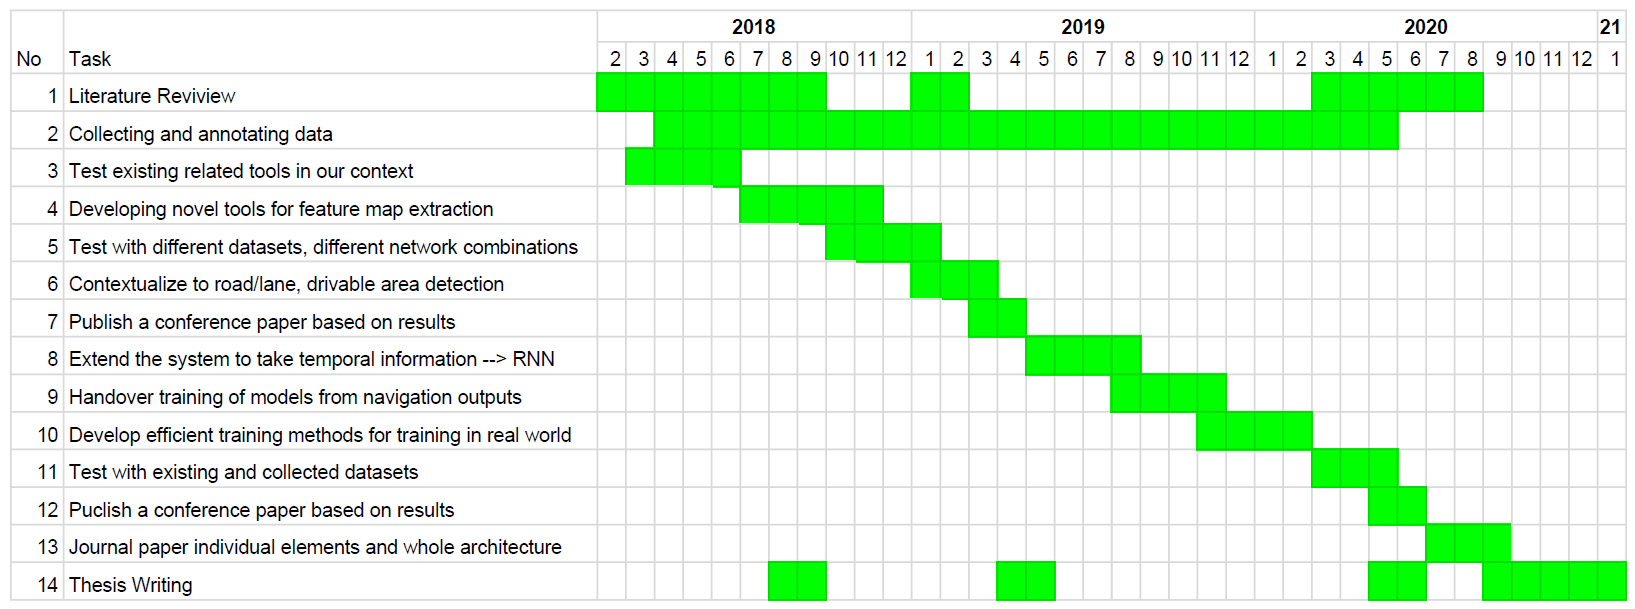
\includegraphics[width=\linewidth]{figures/timeline.png}
	\caption{Work Plan}
	\label{fig:workplan}
\end{figure}


\section{Resource Requirement}
\label{sec:resourcereq}

\begin{enumerate}
\item GPU server 
\item High performance single board computers
\item Large scale dataset for ground vehicles in Sri Lankan context
\item Large scale dataset for low flying aerial vehicles following roads

\end{enumerate}

% Image of work plan
%\begin{figure}[h]
%\begin{center}
%\includegraphics[scale = 0.45]{work_plan.png}\\
%\caption{Work Plan.}\label{fi:work_plan}
%\end{center}
%\end{figure}


\chapter{Conclusion}
\label{ch:conlusion}
The intention of this research is twofold. Firstly overcoming the issue of deploying a single adaptive model to similar but slightly different navigation environments which learns from varying environments under varying conditions without affecting its existing knowledge and experience obtained from other environments. Having a single fixed deeper model is inefficient and even though the model after learned from diverse dataset will be able to generalize to all contexts might not producing best results in each context where a smaller model trained from that particular context only might perform better. Secondly training such system from real world diverse data as well as training in real time. 

We highlighted that the above mentioned needs are not yet fully addressed in the literature where existing researches either try to make pre-recorded dataset larger, or make the neural network deeper. Existing approaches to training does not fully solve the problem of training a navigation system in real world. We believe that training an agent in a simulated environment is not the solution since there is a considerable gap between real world and a simulated environment.

The research objectives include building a pure vision based end-to-end architecture for autonomous navigation which is based on conditionally generated contextualized feature maps which are dynamically adaptive to the environment and taking a promising approach to train such system in real world large scale diverse data. The models we develop are required to learn from slightly different environments while maintaining the experience learned from previous environments. Our research is inspired by the biological behavior of these particular tasks. 

To achieve these objectives a comprehensive research methodology was proposed which starts from a critical review of literature and gradually building required tools towards an end-to-end architecture which extracts both spatial and temporal information from the input in order to output navigation commands. Finally these individual tools will be assembled together in order to build the final system. Specific attention will be given to train the system from real world data taking a hybrid approach of existing learning methods. 


\renewcommand{\bibname}{\normalfont\selectfont\normalsize References}
\bibliographystyle{IEEEtran}
\bibliography{reference}
\addcontentsline{toc}{chapter}{References}
\renewcommand{\bibname}{whatever}

\end{document}
